\subsection{Distributed Extent Management System}
\label{sec:cases:azurestore}

We used \psharp to test the \emph{distributed extent management} component of the Windows Azure vNext distributed storage system. This component is responsible for managing the partitioned extent metadata and works as follows.

\subsection{Live Azure Table Migration}

We also used \psharp to test the MigratingTable library, which is capable of transparently migrating a data set between tables in the Windows Azure storage service while an application is accessing the data set.

\begin{figure}[t]
\centering
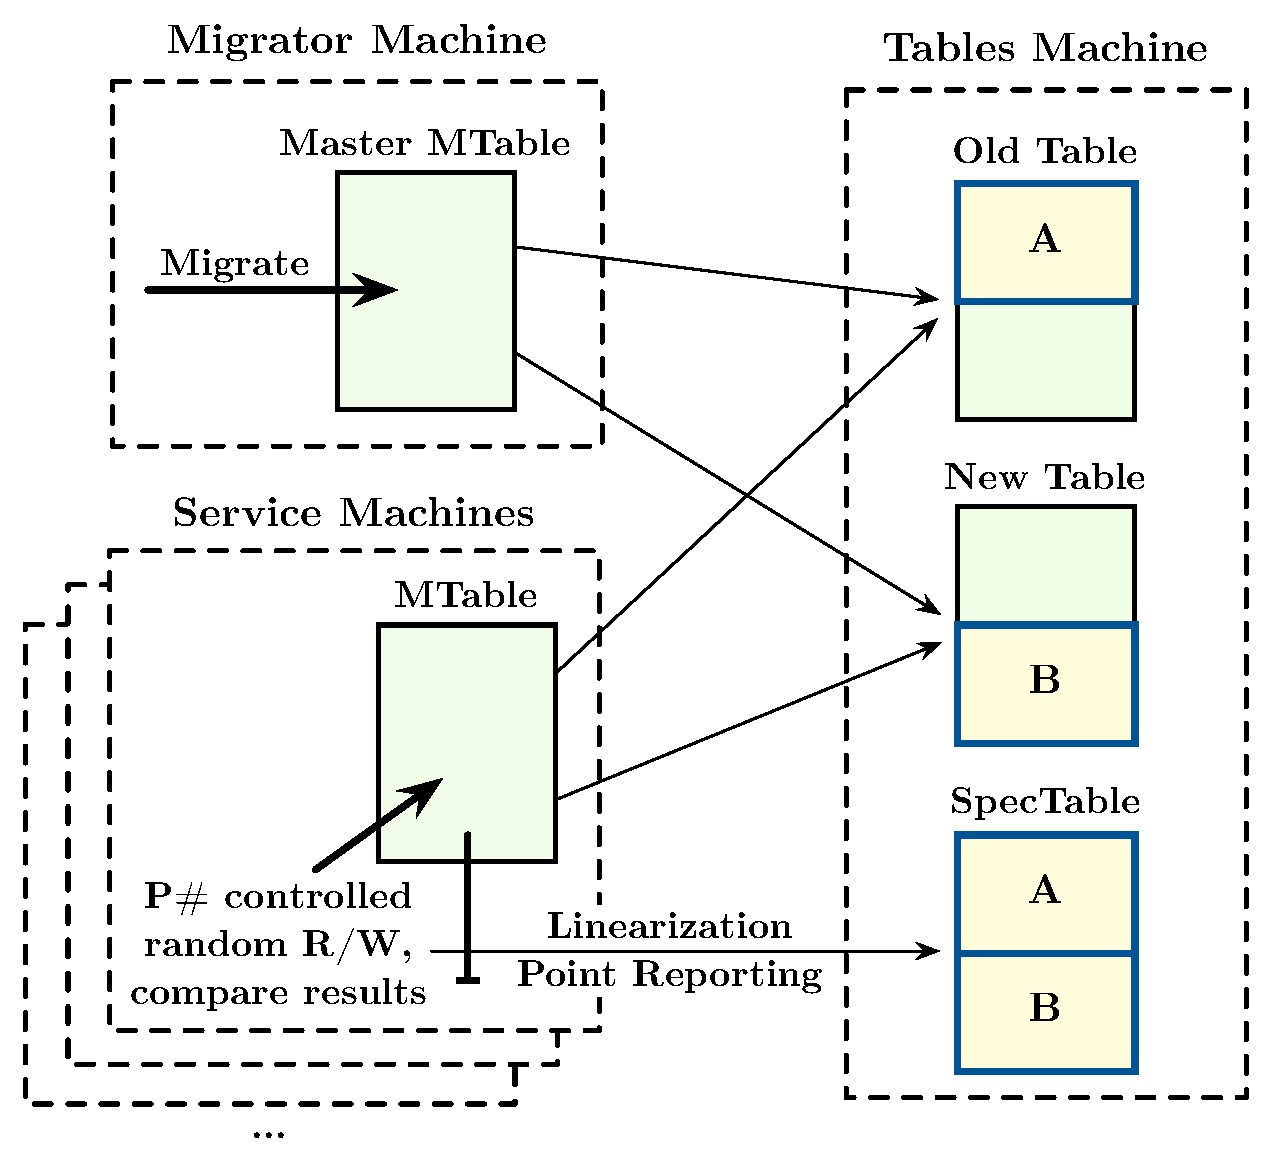
\includegraphics[width=\linewidth]{img/mocked_migration}
\caption{MigratingTable \psharp correctness test environment.}
\label{fig:mockedmigration}
\end{figure}

Since we were designing a new concurrent protocol that we expected to become increasingly complex over time as we add optimizations, we planned from the beginning to maintain a \psharp test harness along with the protocol to maintain confidence in its correctness.

MigratingTable implements an interface called IChainTable2, which provides the core read and write functionality of the real Azure table API with one exception: it provides a weaker consistency property for multi-page reads, since the original property would have been difficult to achieve for no benefit to applications we could foresee.  MigratingTable requires that its backend tables also implement IChainTable2, and we wrote a simple adapter to expose physical Azure tables as IChainTable2.  Our goal was then to verify that when multiple application processes issue ``input'' read and write calls to their own MigratingTable instances with the same backend tables, the behavior complies with the specification of IChainTable2 for the combined input history.

% N.B. SpecTable = InMemoryTableWithHistory in the current codebase. ~ Matt 2015-08-17
Since the specification is deterministic under sequential calls except for the results of multi-page reads, we decided the easiest way to formulate it for automated testing was to write an in-memory reference implementation called SpecTable.  Given a multi-page read, SpecTable can actually produce a list of all valid results.  Our correctness property is then:
\begin{quote}
For every execution trace of a collection of MigratingTables backed by the same pair of SpecTables (which nondeterministically choose one of the valid results for each multi-page read) in parallel with the migrator job, there exists a linearization of the combined input history such that the output in the original trace matches the output of a ``reference'' SpecTable on the linearized input.
\end{quote}
%
\def\term#1{\emph{#1}}
We instrumented MigratingTable to report the \term{linearization point} of each input call, which in our case is always one of the corresponding \term{backend calls} to the backend tables (often the last).  Specifically, after each backend call completes, MigratingTable reports whether it was the linearization point, which may depend on the result of the call.  This makes it possible to verify the correctness property as the system executes.  We have a \psharp \term{tables machine} containing all three SpecTables, a collection of \term{service machines} containing identically configured MigratingTables, and a \term{migrator machine} that performs the background migration (Figure~\ref{fig:mockedmigration}).  Each service machine issues a random sequence of input calls to its MigratingTable, which sends backend calls to the tables machine.  When MigratingTable reports the linearization point of an input call, the service machine sends that input call to the reference table.  When an input call completes, the service machine checks that the results from the MigratingTable and the reference table agree.  \psharp controls the interleaving of the backend calls.  To ensure that the reference table is never observed to be out of sync with the backend tables, after the tables machine processes a backend call, it enters a state that defers further backend calls until MigratingTable has reported whether the backend call was a linearization point and (if so) the call to the reference table has been made.  We use the \psharp nondeterminism API to generate the input calls, so in principle an exhaustive \psharp behavior exploration strategy such as DFS could be used to exhaustively test MigratingTable up to some bound.

% Draft
We wanted to implement the core MigratingTable algorithms in \csharp ``async'' code, like most of Artifact Services.  Async code is readable like traditional procedural code but is translated by the compiler to an event-driven state machine using the Task Parallel Library, gaining most of the performance benefits of that style.  By default, all event processing occurs on the .NET thread pool.

We had to arrange for the continuations to execute within the context of a single \psharp machine, which we did by installing a custom SynchronizationContext.  Then we implemented async RPC between machines in terms of message passing, using RealProxy to avoid most of the marshaling boilerplate.
